\setAuthor{Jaan Kalda}
\setRound{lahtine}
\setYear{2018}
\setNumber{G 3}
\setDifficulty{3}
\setTopic{TODO}

\prob{Ring}
Traadist, mille ühe detsimeetri takistus on üks oom tehakse ring ümbermõõduga kuus detsimeetrit. Iga detsimeetri järel märgitakse punktid $a, b, \ldots, f$. Punktide $a$ ja $e$ vahele ühendatakse patarei pingega \SI{7}{V}, punktide $d$ ja $f$ vahele ampermeeter ning $d$ ja $b$ vahele voltmeeter. Punktid $f$ ja $b$ ühendatakse samast traadist lõigatud kahe-detsimeetrise traadijupiga. Leidke ampermeetri ja voltmeetri näidud.




\hint

\solu
\begin{wrapfigure}[9]{r}{0.4\textwidth}
	\vspace{-30pt}
	\begin{center}
		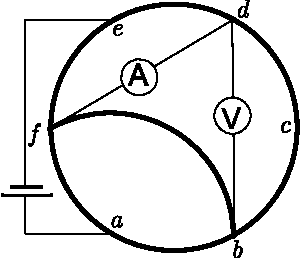
\includegraphics[width = 0.4\textwidth]{2018-lahg-03-yl.pdf}
	\end{center}
\end{wrapfigure}

Teeme ekvivalentskeemi, vt joonis, kus ideaalse ampermeetri asendame traadiga ning ideaalse voltmeetri kõrvaldame. Et voltmeeter on kinnitatud punktide $b$ ja $d$ vahele, siis peame leidma pinge takistil $2R$. Kirhoffi vooluseaduse tõttu näitab ampermeeter ülemise vasakpoolse takisti $R$ ning ülemise takisti $2R$ voolude vahet. Takistus $d$ ja $a$ vahel on takistite $R$ ja $2R$ rööpühendus, st $\frac 23R$ ning $d$ ja $e$ vahel --- $\frac 12R$; seega kogutakistus on $\frac 76R$. Voolutugevus läbi patarei on $I_0=\frac 67\frac{\mathcal E}R$ ning see jaguneb punkte $d$ ja $a$ ühendava ülemise ja alumise haru vahel takistuste suhte vahekorras 1:2, st ülemisse harru läheb vool $I=\frac 13I_0=\frac 27\frac{\mathcal E}R$. Pinge $d$ ja $b$ vahel saame Ohmi seadusest, $U=IR=\frac 27\mathcal E=\SI 2V$. Läbi ülemise vasakpoolse takisti läheb pool koguvoolust, $I_1=\frac 12 I_0=\frac 37\mathcal E$ ja takistit $2R$ läbib vool $I_2=\frac U{2R}= \frac 17\mathcal E$. Seega ampermeeter näitab voolu $I_A=I_2-I_1=\frac{2\mathcal E}{7R}=\SI 2A$.
\probend